\chapter{架构概述}
\label{cha:pipeline}

本章将主要对本人设计的GPU路径渲染平台的架构进行介绍。
首先,由于该平台建立在OpTiX的基础之上,因此会对该库进行简要的说明;
其次将阐述框架的总体设计思路;
最后再逐一对框架的各个组成部分进行分析。

\section{OpTiX库介绍}

OpTiX的本质是一个建立在通用并行语言CUDA上的光线追踪库。图\ref{optix}直观地展示了其内部的工作原理:

\begin{figure}[h]
    \centering
    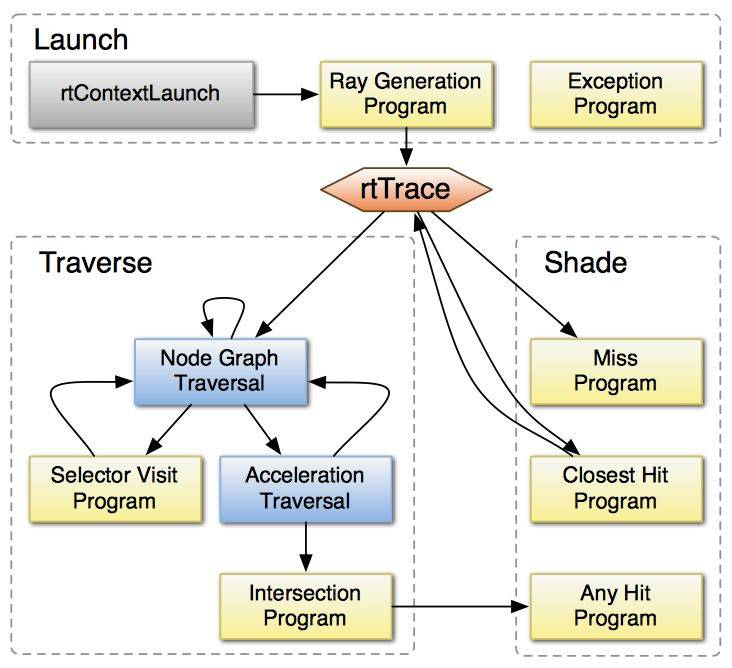
\includegraphics[width=0.6\textwidth]{optix.jpg}
    \caption{OpTiX架构图}
    \label{tab:optix}
\end{figure}

在上图中,黄色的方框代表需要用户自己编写的CUDA程序,蓝色和灰色的部分则由OpTiX实现。
在用户通过调用rtContextLaunch开始渲染后,GPU便会启动其处理单元运行入口函数Ray Generation Program,同时向它们分配互不相同的索引编号。
入口函数需要按照索引值(通常和对应像素的坐标值一致)计算出发射的光线,接着调用rtTrace函数接口开始光线追踪流程。

对于每一根光线,OpTiX会在描述场景的结构图(Node Graph)中进行遍历,从而找到与之相交的物体。
在这其中,Node Graph Traversal负责递归查找,Acceleration Traversal负责利用包围盒等算法为求交过程加速,
而Selecor Visit Program则是由用户添加的一些遍历规则(本文中没有使用)。
如果某条光线和场景中一个物体的包围盒相交,系统便会进一步进入Intersection Program阶段,判断光线与物体是否相交。
如果相交,系统会将该相交事件进行记录,同时调用一次与该物体相关的Any Hit Program。

在所有物体都完成遍历之后,如果没有任何相交出现,系统会调用一次Miss Program,否则针对最近的相交再调用一次Closest Hit Program。
在以上的三个函数中(对应图中的Shade部分),都可以再次调用rtTrace函数,从而进入光线追踪的下一层递归。
最后,如果在以上的任何步骤中出现了诸如栈溢出、违法防存的情况,则会立即终止所有程序,并直接调用Exception Program。
关于函数调用的情况大致便是这样。

除了运行流程外,还需要对OpTiX的几个重要数据结构(以OpTiX Prime++为准)进行介绍。

首先要介绍的是\textbf{Context}(上下文)类。顾名思义,\textbf{Context}类是Host程序(即通过CPU运行的C++程序)和内核程序(运行在GPU上的CUDA程序)之间的桥梁。
Host程序需要将运行所需的所有数据、函数信息一并输入进该类的实际对象中,然后再通过调用这一对象的launch方法开始渲染。
在上述的几个CUDA程序中,Ray Generation Program和Miss Program是与\textbf{Context}直接进行绑定的。

\label{GeometryInstance}
其次是\textbf{GeometryInstance}(几何物体)类和\textbf{Material}(材质)类,前者表示场景中的各个物体,后者则对应着这些物体的材质。
\textbf{GeometryInstance}类在创建实例时需要绑定一个Intersection函数和Bound函数,分别用于该物体的求交计算和包围盒计算。
\textbf{Material}类则需要绑定一个Closest Hit Program函数和一个Any Hit Program函数。
此外,\textbf{GeometryInstance}实例需要包含一个或多个\textbf{Material}对象,当光线与之相交时,会由Intersection函数选择其中一个材质,
然后调用它所绑定的两个Hit Program。

对于上述介绍的三种类型(\textbf{Context},\textbf{GeometryInstance},\textbf{Material}),除去由OpTiX制定的输入参数外,用户还可以往其内部添加一些自定义数据。
这类数据的组织方式与Python语言中的Dict类似,采用以字符串为下标的哈希表维护。
自定义数据支持的格式包括但不限于:基本类型(int, float等)、向量类型(float3, matrix等)、
缓存数据(Buffer类)、以及自定义函数(Program类)。不得不提的是,自定义函数的加入为在GPU中实现运算方法多态性提供了可能,
这在后面的实现中有着相当重要的作用。

另外,本框架还使用到了\textbf{GeometryGroup,Transform,Buffer,Program}等许多其他数据结构,但在这里不再详细进行介绍。

\section{总体架构}
 
从需求上来说,本人期望实现的渲染器能够支持以下几个主要功能:

\begin{itemize}
    \item{能读取不同种类的场景文件}
    \item{拥有图形界面,能够进行交互式渲染}
    \item{能够支持多种不同的几何体、材质、摄像机以及渲染算法}
    \item{支持在线修改场景,并能够实现动画效果}
\end{itemize}

根据这些要求,本文在先后参考了PBRT\cite{pharr2016physically}渲染器,及由Nvidia发布的OpTiX样例程序等多方材料后,
最终设计了如图\ref{tab:framework}所示的架构:


\begin{figure}[h]
    \centering
    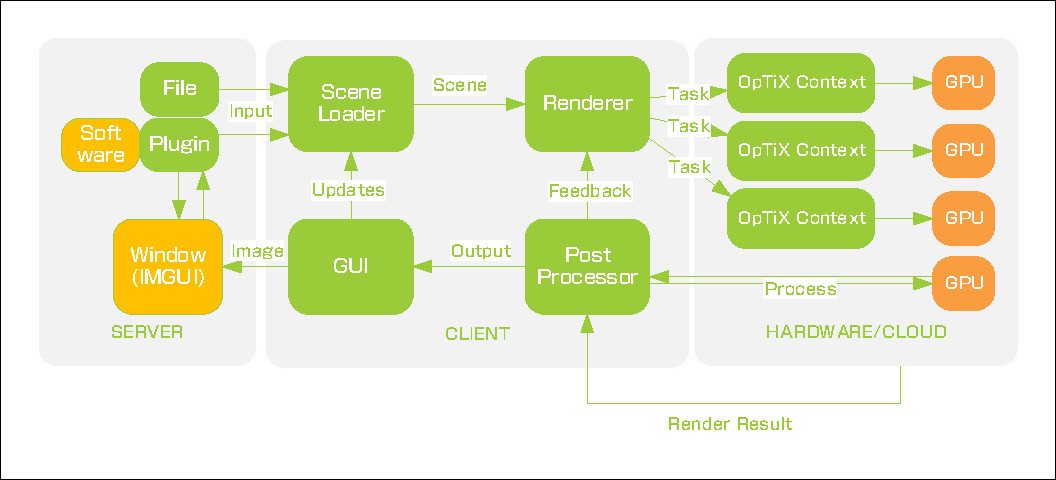
\includegraphics[width=\textwidth]{Framework.pdf}
    \caption{(TODO:图片还有些问题)GPU渲染器的总体架构。在该架构中,用户可以通过场景文件或三位建模软件插件向渲染器提供场景,
    在渲染器(即图中SERVER、HARDWARE/CLOUD部分)完成渲染后,会将结果通过图形界面进行显示,并为用户提供用于修改场景的交互平台。}
    \label{tab:framework}
\end{figure}

总体而言,该框架一共由四个模块组成:\textbf{\textbf{Scene}},\textbf{Renderer},\textbf{PostProcessor}以及\textbf{GUI}。其中,
\textbf{\textbf{Scene}}的功能是将不同种类的输入场景文件进行读取,以及把数据转化成可被OpTiX使用的中间格式;
\textbf{Renderer}的功能是建立并配置OpTiX中的\textbf{Context}类,将\textbf{\textbf{Scene}}中的所有数据输入到\textbf{Context}中,以及调用launch方法完成渲染工作;
\textbf{PostProcessor}的功能是对\textbf{Renderer}的输出图像进行后处理,以及根据优化算法向\textbf{Renderer}提供反馈信息;
最后,\textbf{GUI}负责的是图形界面部分,将处理出来的图像展示到屏幕中,并处理由用户传来的交互数据。

除了模块结构外,本框架还制定了一套完整的工作流程:

\begin{enumerate}
    \item{用户启动渲染器,输入场景文件以及渲染全局参数;}
    \item{根据输入的场景文件格式,建立\textbf{\textbf{Scene}}模块对文件进行解析;}
    \item{根据输入的全局参数,建立\textbf{Renderer},并生成\textbf{Context};}
    \item{将\textbf{\textbf{Scene}}中的数据,以及全局参数提供给\textbf{Context};}
    \item{建立\textbf{GUI},初始化渲染结果,然后开始以下循环:}
    \begin{enumerate}[\arabic{enumi}.1]
        \item{启动\textbf{Renderer}完成一轮渲染,并将结果进行累加;}
        \item{将累计结果输入\textbf{PostProcessor}进行后处理;}
        \item{显示\textbf{PostProcessor}的输出图像,同时向\textbf{Renderer}提交反馈;}
        \item{监控用户操作,如果场景或参数出现改动,则跳至第4步;}
    \end{enumerate}
    \item{保存结果,退出程序。}
\end{enumerate}

以上便是关于该架构的总体情况。下面将按照四个模块在流程中出现的顺序,依次对它们的设计细节进行阐述。
需要注意的是,本章后面的内容为了可能会为了扩展功能而对前面的结构进行修正,
因此框架的最终形式以本章结束时的版本为准。

\section{场景读取与载入}

载入场景往往是一般渲染流程中工作量最为庞大的步骤之一,而对于GPU渲染器来说,这一步则显得更加困难。
这是因为,在从输入文件中读取数据的同时,我们还需要考虑如何将这些数据有效地组织起来,
从而使得GPU中的程序对不同种类的场景都能提供支持。
为了达到这点要求,我们首先便需要分析一个场景应当由哪些部分组成:

\label{PropertyList}
\begin{itemize}
\item{各个物体的几何模型}
\item{物体上的材质属性(包括贴图)} 
\item{场景中不同介质的属性} 
\item{光源属性}
\item{相机属性}
\item{以上所有属性在时域上的变化情况(动画属性)}  
\end{itemize}

在OpTiX内的渲染流程中,以上这些数据的使用程序各有不同。
物体的几何模型主要在物体的两个求交函数中被用到;
材质属性、介质属性以及光源属性会在Closest Hit、Any Hit以及Ray Generation三类程序中得到使用;
摄像机的属性只会被用于Ray Generation程序;
由于动画可以放在Host程序里面实现,因此动画属性不涉及任何GPU程序。
根据这些属性的应用范围,本架构使用了三种不同的抽象类\textbf{Geometry、Property、Animator}对它们进行描述。
其中,\textbf{Geometry}类用于几何模型;
\textbf{Property}类用于几何外的所有静态属性——材质、介质、光源、摄像机;
\textbf{Animator}类则用于动画属性。
下面是对这三类的介绍。

\subsection{几何模型——Geometry}


\begin{figure}[h]
    \centering
    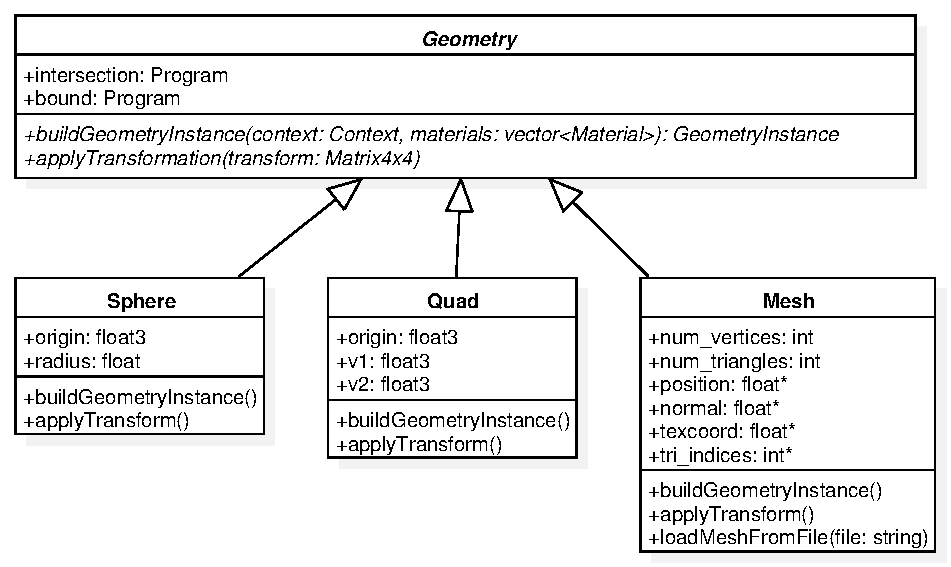
\includegraphics[width=0.8\textwidth]{Geometry.pdf}
    \caption{\textbf{Geometry}类的内部结构}
    \label{tab:geometry}
\end{figure}

我们不妨从OpTiX的角度来考虑应当如何设计\textbf{Geometry}类。
根据\ref{GeometryInstance}中的内容,在OpTiX中建立一个\textbf{GeometryInstance}实例需要提供三种数据:
两个用于求交的函数(\textbf{Program})、描述几何模型的参数(自定义参数)以及物体的材质(\textbf{Material})。
可以发现,用于求交的函数往往只与集合体的种类相关,因此这里看作是\textbf{Geometry}各个子类的静态成员变量。
几何模型的参数直接作为$\textbf{Geometry}$的成员变量。
至于材质\textbf{Material},则直接由它的上级结构$\textbf{Scene}$来提供,这里不做维护。

综合上述内容,\textbf{Geometry}向外提供了一个直接生成\textbf{GeometryInstance}的接口buildGeometryInstance。
另外,由于在一些场合中需要对\textbf{Geometry}中的几何参数进行空间变换,因此还需要提供一个applyTransform接口。

\lstset{language=C++}
\begin{lstlisting}
virtual GeometryInstance buildGeometryInstance(Context&, vector<Material>&);
virtual void applyTransform(Matrix4x4&);
\end{lstlisting}

\subsection{场景属性——Property}

\begin{figure}[h]
    \centering
    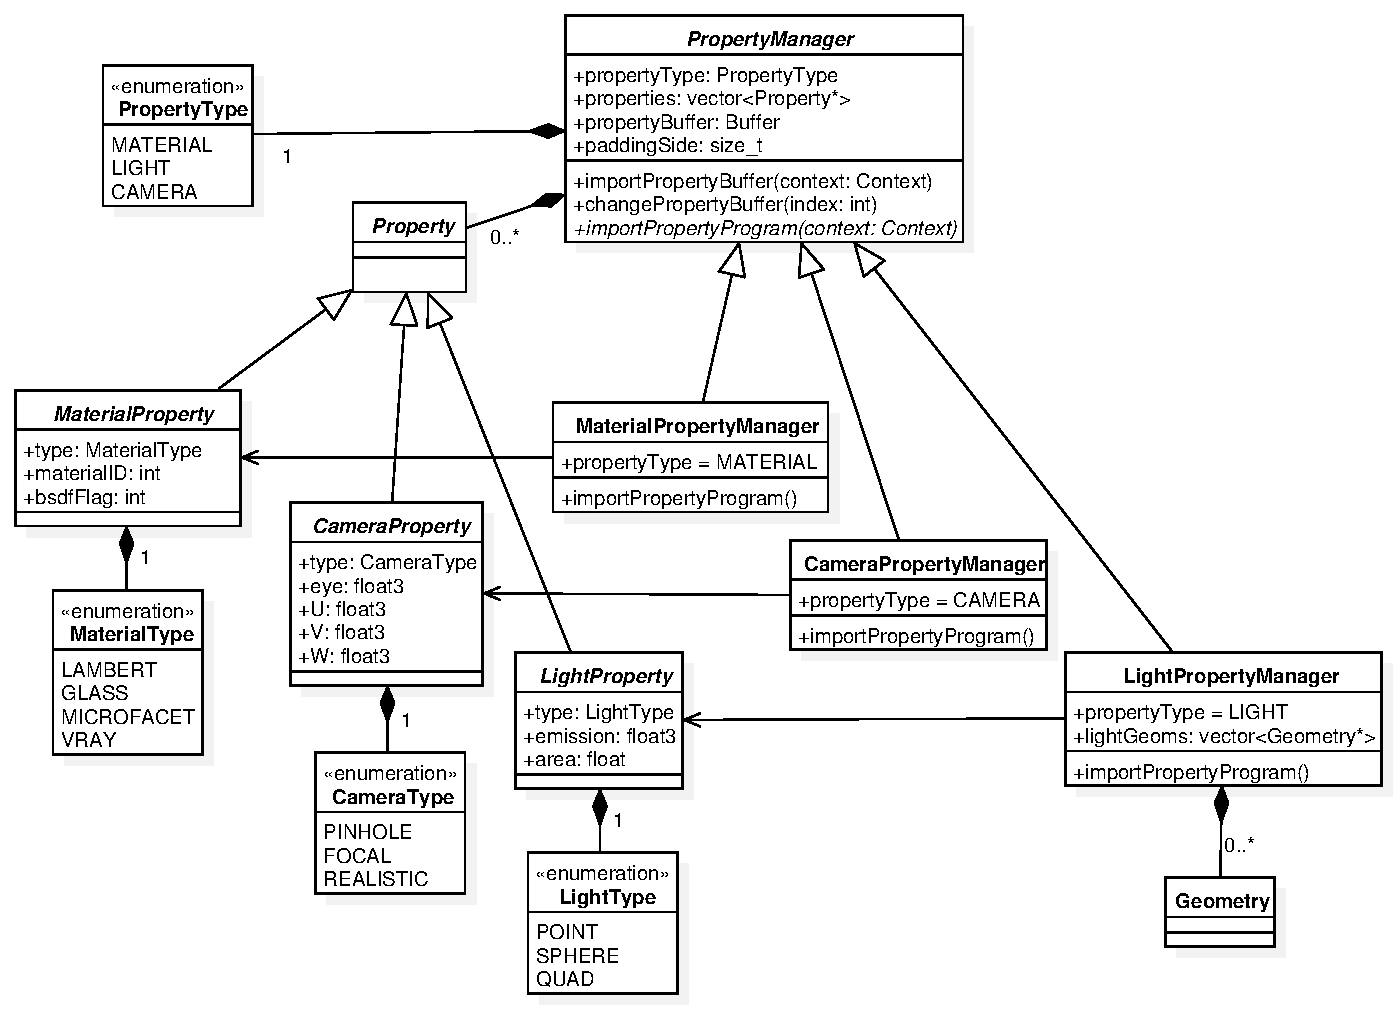
\includegraphics[width=\textwidth]{Property.pdf}
    \caption{\textbf{Property}类及\textbf{PropertyManager}类的内部结构。
    \textbf{Property}类和\textbf{PropertyManager}类分别都拥有不同的几个子类,以代表不同的场景属性,
    但所有\textbf{PropertyManager}的子类都只包含\textbf{Property}抽象类本身(而非对应的子类),
    这主要是为了在实现其函数方法时能够简化代码。
    另外,由于空间限制,图中没有画出所有\textbf{Property}子类的子类,以及目前未在代码中实现的\textbf{MeduimProperty}类。}
    \label{tab:property}
\end{figure}

Property类是在场景输入当中最为重要的一环,它所解决的问题,是如何将不同种类的场景属性按照尽可能一致地格式输入进OpTiX中,从而使得所需的代码量达到最少。
这些属性往往由两部分组成,第一部分是数据,另一部分则是不同属性种类对应的计算函数。
举例来说,对于物体的材质而言,GPU中的内核程序既需要知道材质的各种参数(如颜色、反射率、光泽度等),
也需知道如何利用这些参数计算BRDF值,如何进行采样等等。
由于在GPU程序中,既不能通过指针的方式做到数据多态,也不能通过虚函数的方式实现函数多态。
所以,在这里只能采用更加初级的方法来解决问题。

关于数据部分,有一种思路看起来似乎非常直接:和\textbf{Geometry}的处理方式一样,利用OpTiX中添加自定义数据的方法来完成输入。
但是,本人最终没有采用这种方式,理由主要有两点(以材质属性为例):第一,如果采用这种方案,材质属性应该被绑定在它所对应的\textbf{Material}中。
然而在一些渲染算法如SPPM里,Ray Generation程序也需要使用到这些属性,但却无法直接访问\textbf{Material},因此会产生矛盾;
第二,如果采用了这种方案,则不同种类的\textbf{Material}必须分别配置各自的Closest Hit Program以使用该类型的属性,
这会使得代码量变得十分巨大。相比之下,本框架所采用的方法则要显得轻便许多。

本人最终采用的是通过\textbf{Buffer}类来进行输入的方法。
在OpTiX中,\textbf{Buffer}能够以数组的形式向内核程序传递任意类型的数据,但要求数组中所有元素的格式保持一致。
这里本人采用了填充(Padding)的方式来对数据进行对齐。本人为\textbf{Property}添加一个新的子类\textbf{PaddingProperty},
保证其大小超过所有\textbf{Property}中的最大长度,用它作为\textbf{Buffer}的数据类型。
对于内核程序而言,在从\textbf{Buffer}中拿到一个\textbf{PaddingProperty}类时,程序只需要知道它的真实类型(包含在\textbf{Property}部分中),
然后进行一次格式强制转换,便可以获得实际输入的数据了。


接下来是如何对\textbf{Property}的计算函数实现重载。这里本框架采用的是函数指针的方式。
在OpTiX中,函数指针实际是通过函数ID(rtCallableProgramId)这个数据结构来表示的,而它同样也是\textbf{Buffer}支持的数据类型之一。
在渲染开始之前,Host程序会依次求得所有可能出现的计算函数的函数ID,然后将其保存在对应的\textbf{Buffer}之中;
而在渲染过程中,内核程序只需要知道属性的类型,便可以在\textbf{Buffer}里面查到该属性对应的计算函数了。

按照小节\ref{PropertyList}中提出的四种不同属性,Property一共拥有四个子类:\textbf{\textbf{Material}Property},\textbf{LightProerty},\textbf{CameraProperty}以及\textbf{MediumProperty}。
这四者在结构上基本保持一致,它们又拥有着属于各自的子类。限于篇幅,有关这些不同Property的内部实现,这里便不再进行逐一介绍。

最后需要提到的一点是,和\textbf{Geometry}不同,\textbf{Property}作为数据结构,需要直接出现在内核程序之中。
然而,将这些\textbf{Property}输入OpTiX的方法(比如说生成\textbf{Material})却涉及到OpTiX的Host代码,因此不能被引入内核程序,这就引发了矛盾。
为了解决这个问题,本人在此又加入了一个新的类\textbf{PropertyManager},
用来管理场景中所有的\textbf{Property}类,同时封装与\textbf{Property}相关的Host程序。\textbf{PropertyManager}一共提供了三个函数接口:

\lstset{language=C++}
\begin{lstlisting}
void importPropertyBuffer(Context);
void changePropertyBuffer(int);
virtual void importPropertyProgram(Context);
\end{lstlisting}

其中,importPropertyBuffer函数将已有的\textbf{Property}(保存在\textbf{PropertyManager}中)通过填充方法放入\textbf{Buffer}之中;
changePropertyBuffer函数会将指定下标的\textbf{Property}数据上传给\textbf{Buffer};
而importPropertyProgram函数则负责把与\textbf{Property}相关的所有计算函数一起输入OpTiX中。
和\textbf{Property}一样,\textbf{PropertyManager}也有着相应的四个子类,这些子类之间有着更大的差异(如\textbf{LightPropertyManager}还会维护光源的\textbf{Geometry}列表)
且都没有再被进一步继承下去。

\subsection{动画——Animator}

\textbf{Animator}类的主要作用是记录场景内的所有属性随时间变化的情况。
当系统给定一个时间值时,\textbf{Animator}的任务便是计算场景中各个属性在该时间下的值。

问题的关键在于,如何能让不同种类的属性(\textbf{Geometry}和\textbf{Property})都能拥有各自的动画属性。
一种解决的思路是对于这些属性,都创建一个对应的\textbf{Animator}子类,
然后通过这些子类的接口函数进行修改。
然而这样的做法会让代码量变得十分巨大,而且不利于在将来进行拓展。
本框架中采用的方法,则是将\textbf{Animator}的粒度缩小到了基本类型上(如int,float,float3等),
而由不同的属性自己组装这些\textbf{Animator}从而实现动画。
在代码实现上,只需要在\textbf{Geometry}和\textbf{Property}中
加入一个由\textbf{Animator}指针组成的数组(每一个\textbf{Animator}都对应属性中的一个变量),
再添加一个接口函数setTime来遍历这些\textbf{Animator}即可。
\lstset{language=C++}
\begin{lstlisting}
bool setTime(float);
\end{lstlisting}

至于\textbf{Animator}类本身的情况,总体来说,它通过继承来实现不同的计算方式(线性差值、Bezier曲线等等),
而通过模板方法实现对各种基本类型的支持。该类只需要提供一个接口函数:
\lstset{language=C++}
\begin{lstlisting}
T getAnimationByTime<T>(float);
\end{lstlisting}



\subsection{场景——Scene}

\begin{figure}[h]
    \centering
    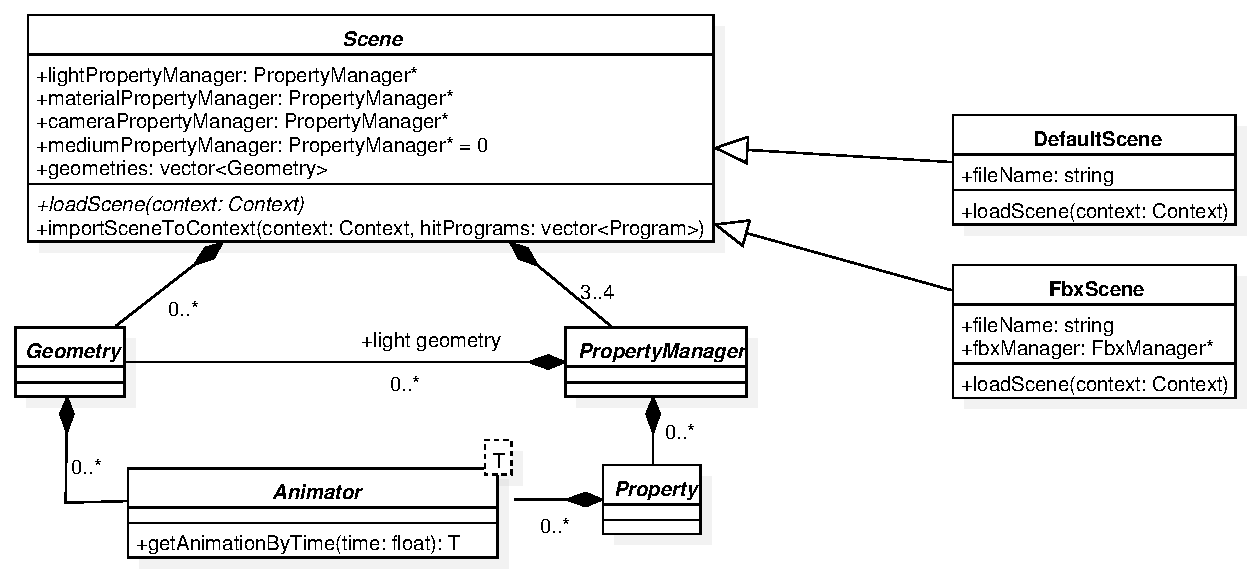
\includegraphics[width=\textwidth]{Scene.pdf}
    \caption{\textbf{Scene}类的内部结构。注意该图中引入了上一章介绍的\textbf{Animator}类,
    该类是一个带模板参数的抽象类,其各个子类分别对应了不同的动画计算方法(又称策略)。}
    \label{tab:scene}
\end{figure}

\textbf{Scene}类表示的是整个场景中的所有信息。从之前列举的场景内容来看,
它需要包含一个\textbf{Geometry}组成的数组,和四种不同的\textbf{PropertyManager}。
在功能上,它应当支持两个操作:从文件中读取数据,以及将数据放入到OpTiX的\textbf{Context}中。这两个操作对应的接口函数为:
\lstset{language=C++}
\begin{lstlisting}
virtual void loadScene(Context);
virtual void importSceneToContext(Context, vector<Program>&);
\end{lstlisting}

这里有两点需要做出特殊说明。首先,从设计上来讲,在读取文件的时候不应当需要使用\textbf{Context}作为参数,
但这里加入\textbf{Context},主要是为了在一些地方(如Mesh读取出)提前获取\textbf{Buffer}的地址,从而避免在读取完后再将数据拷贝到这些\textbf{Buffer}中;
其次第二个函数的参数中加入了一个\textbf{Program}数组,这些\textbf{Program}实际是由之后介绍的\textbf{Renderer}所确定的Closest Hit Program和Any Hit Program,
由于这两者必须被绑定到由\textbf{MaterialPropertyManager}生成的\textbf{Material}上,所以这里它们也需要作为参数被传进来。

\section{渲染器——Renderer}

\begin{figure}[h]
    \centering
    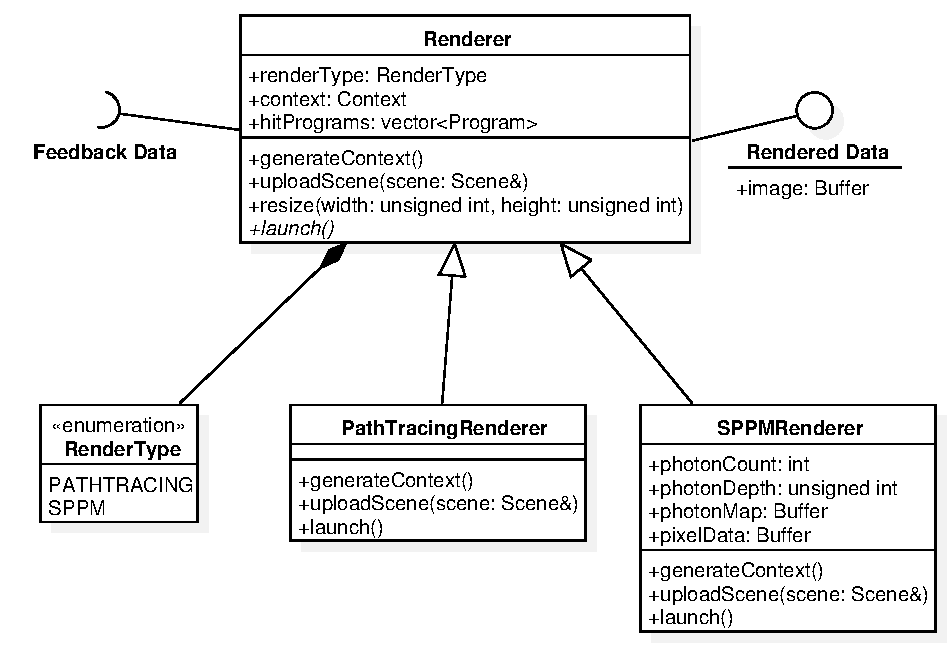
\includegraphics[width=0.7\textwidth]{Renderer.pdf}
    \caption{\textbf{Renderer}类的内部结构。\textbf{Renderer}类需要支持两个数据接口,
    一个是渲染生成的图像输出和其他场景信息(Rendered Data),另一个则是输入的反馈信息(Feedback Data)。}
    \label{tab:renderer}
\end{figure}

\textbf{Renderer}类的主要任务是生成并初始化\textbf{Context},及完成渲染工作。事实上,有了之前\textbf{Scene}的基础,它在实现上相对简单许多。
\textbf{Renderer}需要维护的数据包括但不限于由它生成的\textbf{Context},与渲染算法相关的Hit Program,以及所有用于渲染的输入、输出\textbf{Buffer}。
此外,它还需要支持以下的四个接口函数:

\lstset{language=C++}
\begin{lstlisting}
virtual void generateContext();
virtual void uploadScene(Scene&);
virtual void resize(uint, uint);
virtual void launch();
\end{lstlisting}

generateContext函数的功能便是是建立一个\textbf{Context}。为了这个\textbf{Context}能够运转,在该函数中还要根据不同的渲染算法,
设定\textbf{Context}的全局参数、创建输入输出的\textbf{Buffer}、以及为\textbf{Context}指定Ray Generation、Exception和Miss三种程序。
该函数还会生成与渲染算法相关的Closest Hit Program与Any Hit Program。

uploadScene函数的主要作用的是调用上述\textbf{Scene}中的importSceneToContext函数来完成场景读入,除此之外,
一些需要根据\textbf{Scene}的参数(如包围盒大小)来决定的\textbf{Renderer}参数也会在这里进行设置。

resize函数用来修改渲染器的渲染尺寸,以支持用户对窗口进行放缩的操作。
具体内容主要包括修改相机参数、各种图像Buffer的尺寸大小等等。

最后也是最为重要的是函数launch,其功能便是用OpTiX完成一轮渲染。
在这个函数中,将会一次或多次调用\textbf{Context}的launch接口,启动OpTiX的GPU渲染程序。
在下一章GPU光线追踪渲染算法的介绍中,对这个函数内部的实现会展开更细致的说明。

\section{图像后处理——PostProcessor}

\begin{figure}[h]
    \centering
    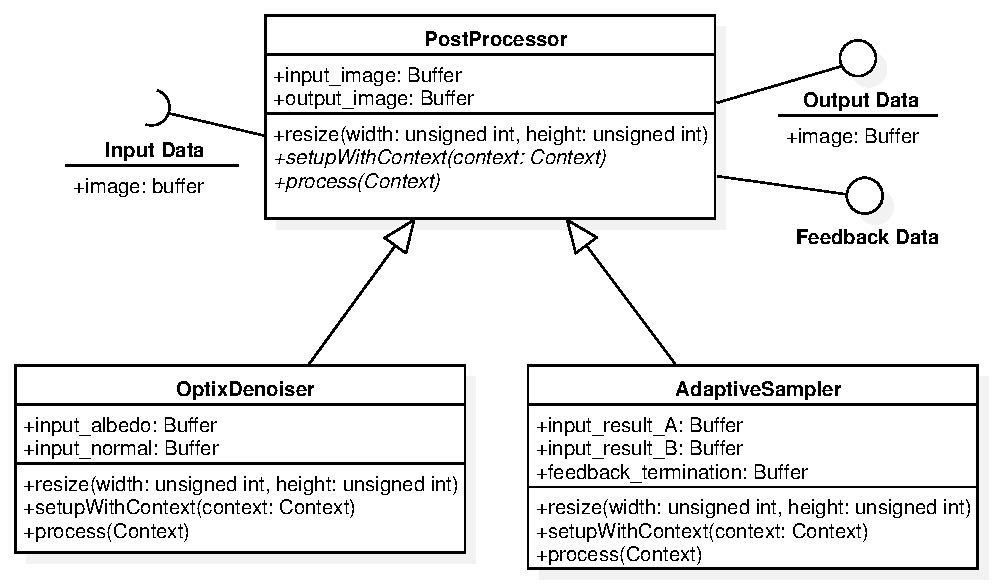
\includegraphics[width=0.7\textwidth]{PostProcessor.pdf}
    \caption{\textbf{PostProcessor}类的内部结构,和\textbf{Renderer}类相似,
    该类需要支持一个输入数据接口,一个输出数据接口,和需要传递给\textbf{Renderer}的反馈数据接口。}
    \label{tab:postprocessor}
\end{figure}

\textbf{PostProcessor}负责将\textbf{Renderer}的输出图形进行后处理,然后再将一些信息反馈回\textbf{Renderer}。
他的构造非常简单,由一个输入\textbf{Buffer},一个输出\textbf{Buffer},以及所有的辅助数据(包括反馈、由渲染器提供的其他信息)组成。
它需要实现三个接口函数:

\lstset{language=C++}
\begin{lstlisting}
virtual void setupWithContext(Context&);
virtual void resize(uint, uint);
virtual void process(Context&);
\end{lstlisting}

简单来说,setupWithContext函数负责对该处理器进行初始化,resize函数和之前一样用于修改尺寸,
而process函数便是完成一次后处理操作。用户创建一个后处理器实例后,首先要手动制定其输入\textbf{Buffer},
然后调用初始化函数便会生成输出\textbf{Buffer}和其它的辅助数据。
这些数据可以作为最终输出,可以接回\textbf{Renderer},也可以再接到后续的后处理器上。

另外需要注意的是,对于有反馈的后处理算法而言,\textbf{Renderer}也需要做出相应的修改以提供支持。
一种比较合理的解决方法是采用Decorator设计模式,通过引入\textbf{Renderer}的修饰类来达到这一目标。
但由于渲染算法的修改通常都需要深入到OpTiX的内核程序中去,因此在这个过程中有许多代码是不可避免地需要重写的。

\section{图形界面——GUI}

\begin{figure}[h]
    \centering
    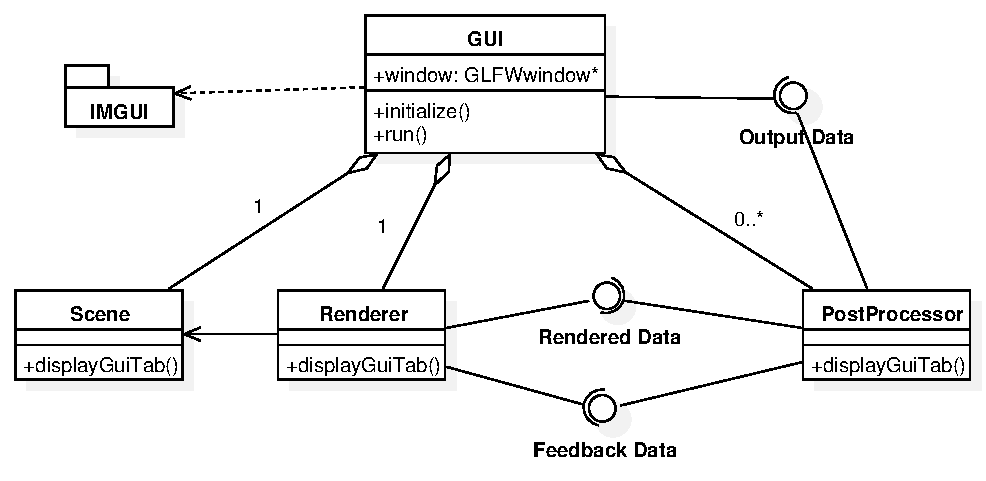
\includegraphics[width=\textwidth]{GUI.pdf}
    \caption{GUI类的内部结构,包括\textbf{Renderer}类和\textbf{PostProcessor}类的接口链接方式。}
    \label{tab:gui}
\end{figure}


\textbf{GUI}类是整个流程当中的最后一个被创建的模块,负责与用户之间的一切交互。
它主要需要包含三个功能:运行完整的渲染流程、显示结果、以及接受用户的各种修改操作。

\textbf{GUI}类拥有一个\textbf{Scene}的指针,一个\textbf{Renderer}的指针
以及一个由\textbf{PostProcess}的指针组成的数组。这三者包含了有关渲染器的全部信息。
它的主要接口函数则有两个:
\lstset{language=C++}
\begin{lstlisting}
void initialize();
void run();
\end{lstlisting}

用户首先需要调用initialization函数初始化\textbf{GUI}(主要是初始化其底层支持的库如glfw等),
然后将生成的\textbf{Scene}、\textbf{Renderer}等其他模块逐个输入进\textbf{GUI}中,
最后调用run函数开始循环。

\textbf{GUI}类的具体实现是基于Dear ImGui图形界面库\footnote{https://github.com/ocornut/imgui}(以下称为ImGui)完成的。该界面库拥有扩展性强,简单轻便的特点,
因此很方便用来实现用户的交互操作。在本人的设计框架中,用户一共可以进行四种类型的操作:修改窗口的大小;修改当前时间(用于动画);
通过鼠标拖拽修改相机位置;通过固定表项修改场景属性(或渲染属性)。
关于修改窗口大小、修改时间的操作,只需要直接调用之前介绍的方法即可完成。
其余两种操作则在实现上更为复杂。

首先说如何修改相机位置。当ImGui检测到鼠标事件后,后台需要根据事件的具体情况来计算出新的相机位置,然后将其输入到OpTiX中。
可以发现,\textbf{CameraPropertyManager}类正好适合于完成这样的工作。因此,本人在该类中又增加了一个新的接口函数:

\lstset{language=C++}
\begin{lstlisting}
void processMouse(float, float, bool, bool, bool, float);
\end{lstlisting}

该函数的参数均为描述鼠标事件的变量。它在计算完新的相机信息后,
只需直接调用本类的changePropertyBuffer函数便完成了对OpTiX的数据更新。

其次来说场景属性的修改。对于这一部分而言,最主要的问题是如何为不同类型的属性生成相应的表项。
这里采用的方法是:通过递归算法遍历场景中每个属性对应的实例,然后由这些对象自行向ImGui提出所需的表项。
为此,之前提到的所有类(\textbf{Geometry}、\textbf{Property}、\textbf{PropertyManager}、\textbf{Scene}、\textbf{Renderer}、\textbf{PostProcessor})都需要再添加一个接口函数:
\lstset{language=C++}
\begin{lstlisting}
virtual bool displayGuiTab() 
\end{lstlisting}

该函数会调用ImGui的方法来进行声明,而ImGui则会对这些声明统一记录起来。
最终,ImGui会将所有被记录的表项都一次性输出在图形窗口上。
该函数需要返回一个Bool值,用来表示该表项是否被修改过(从ImGui的声明函数中直接获得),
该值可以用于决定是否要对OpTiX上的数据进行更新。
